\documentclass[a4paper,11pt]{article}

% Set page size and margins
\usepackage[a4paper,top=2cm,bottom=2cm,left=3cm,right=3cm,marginparwidth=1.75cm]{geometry}

%Karnaugh Maps
\usepackage{karnaugh-map}

% TOC
\usepackage{titlesec}

% Lists
\usepackage{enumitem}

% Tables
\usepackage{tabularx}

% Code rendering
\usepackage{listings}

% Useful packages
\usepackage{amsmath}
\usepackage{mathtools}
\usepackage{graphicx}
\usepackage[colorlinks=true,linkcolor={black},citecolor={blue!80!black},urlcolor={blue!80!black}]{hyperref}

% Custom shorthands
%% Table cmds
\newcommand\HSPC{\rule{0pt}{4ex}\rule[-2.0ex]{0pt}{0pt}}
\newcommand\RSPC{\rule{0pt}{2.5ex}\rule[-1.25ex]{0pt}{0pt}}

%% Math cmds
\newcommand{\mathfsc}[2]{#1#2\normalsize}

% Code bloc styling
\lstdefinestyle{myStyle}{
    breaklines=true,
    frame=single,
    numbers=left,
    numbersep=10pt,
    numberstyle=\normalsize\color{gray!80!black},
    basicstyle=\large\ttfamily,
    keywordstyle=\bfseries\color[HTML]{FE4A49},
    commentstyle=\itshape\color[HTML]{A6A6A8},
    identifierstyle=\color[HTML]{2AB7CA},
    backgroundcolor=\color[HTML]{F4F4F8},
    stringstyle=\color[HTML]{FED766}
}


\title{\textbf{ GATE QUESTION SOLUTION }}
\author{AKANKSHA MORE}

\begin{document}
\date{}
\maketitle

% Make Table of contents from Sections
\tableofcontents

% Problem Statement
\newpage
\section{Problem}
\label{sec:ques}
\textbf{(GATE CS Q55(a)- YEAR 2002)}\\
\textbf{Q.55(a)}: Express the function f(x,y,z)=xy'+yz' with only one complement operation and one or more AND/OR operations.Draw the logic circuit implementing the expression obtained,using a single NOT gate and one or more AND/OR gates.
      \tikzset{every picture/.style={line width=0.75pt}} %set default line width to 0.75pt        
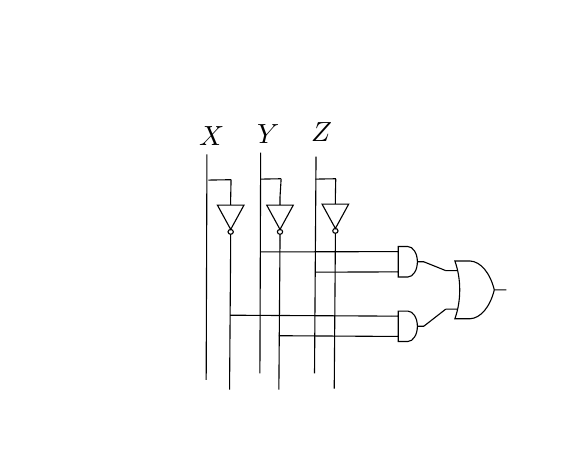
\begin{tikzpicture}[x=0.5pt,y=0.5pt,yscale=-1,xscale=1, baseline=(XXXX.south) ]
\path (0,298);\path (380.5874938964844,0);\draw    ($(current bounding box.center)+(0,0.3em)$) node [anchor=south] (XXXX) {};
%Shape: Not/Inverter Gate [id:dp26042681958505076] 
\draw   (156.31,128.25) -- (146.72,145.81) -- (137.13,128.25) -- (156.31,128.25) -- cycle (146.72,122.4) -- (146.72,128.25) (146.72,149.32) -- (146.72,154) (146.72,145.81) .. controls (147.78,145.81) and (148.64,146.59) .. (148.64,147.56) .. controls (148.64,148.53) and (147.78,149.32) .. (146.72,149.32) .. controls (145.66,149.32) and (144.8,148.53) .. (144.8,147.56) .. controls (144.8,146.59) and (145.66,145.81) .. (146.72,145.81) -- cycle ;
%Shape: Not/Inverter Gate [id:dp5398487412826742] 
\draw   (231.97,127.56) -- (222.38,145.11) -- (212.78,127.56) -- (231.97,127.56) -- cycle (222.38,121.7) -- (222.38,127.56) (222.38,148.62) -- (222.38,153.3) (222.38,145.11) .. controls (223.44,145.11) and (224.29,145.9) .. (224.29,146.87) .. controls (224.29,147.84) and (223.44,148.62) .. (222.38,148.62) .. controls (221.32,148.62) and (220.46,147.84) .. (220.46,146.87) .. controls (220.46,145.9) and (221.32,145.11) .. (222.38,145.11) -- cycle ;
%Shape: Not/Inverter Gate [id:dp423577485685779] 
\draw   (191.95,128.25) -- (182.36,145.81) -- (172.76,128.25) -- (191.95,128.25) -- cycle (182.36,122.4) -- (182.36,128.25) (182.36,149.32) -- (182.36,154) (182.36,145.81) .. controls (183.42,145.81) and (184.27,146.59) .. (184.27,147.56) .. controls (184.27,148.53) and (183.42,149.32) .. (182.36,149.32) .. controls (181.3,149.32) and (180.44,148.53) .. (180.44,147.56) .. controls (180.44,146.59) and (181.3,145.81) .. (182.36,145.81) -- cycle ;
%Straight Lines [id:da5844174635722277] 
\draw    (129.55,91.6) -- (129,254.46) ;
%Straight Lines [id:da3443328569890023] 
\draw    (168.38,90.38) -- (167.83,249.77) ;
%Straight Lines [id:da6242253347188811] 
\draw    (208.4,93.17) -- (207.3,249.77) ;
%Straight Lines [id:da8044375364944794] 
\draw    (146.72,154) -- (145.9,261.6) ;
%Straight Lines [id:da9732926819519225] 
\draw    (182.36,154) -- (181.53,261.6) ;
%Straight Lines [id:da023580383561008444] 
\draw    (222.38,153.3) -- (221.55,260.9) ;
%Straight Lines [id:da904908941108862] 
\draw    (130.55,110.15) -- (146.99,109.87) ;
%Straight Lines [id:da5981058842754439] 
\draw    (207.85,109.45) -- (222.65,109.18) ;
%Straight Lines [id:da21470416541921744] 
\draw    (168.38,109.45) -- (183.18,109.18) ;
%Straight Lines [id:da49970717929539776] 
\draw    (146.99,109.87) -- (146.72,122.4) ;
%Straight Lines [id:da22010191891802044] 
\draw    (183.18,109.18) -- (182.36,122.4) ;
%Straight Lines [id:da1916520778758366] 
\draw    (222.65,109.18) -- (222.38,121.7) ;
%Shape: And Gate [id:dp9681906085714931] 
\draw   (267.82,158.17) -- (274.73,158.17) .. controls (278.54,158.17) and (281.64,163.1) .. (281.64,169.17) .. controls (281.64,175.24) and (278.54,180.17) .. (274.73,180.17) -- (267.82,180.17) -- (267.82,158.17) -- cycle (263.22,161.84) -- (267.82,161.84) (263.22,176.5) -- (267.82,176.5) (281.64,169.17) -- (286.24,169.17) ;
%Shape: And Gate [id:dp04793014025244369] 
\draw   (267.82,204.81) -- (274.73,204.81) .. controls (278.54,204.81) and (281.64,209.73) .. (281.64,215.8) .. controls (281.64,221.87) and (278.54,226.8) .. (274.73,226.8) -- (267.82,226.8) -- (267.82,204.81) -- cycle (263.22,208.47) -- (267.82,208.47) (263.22,223.13) -- (267.82,223.13) (281.64,215.8) -- (286.24,215.8) ;
%Shape: Or Gate [id:dp16976140238006088] 
\draw   (308.72,168.61) -- (319.69,168.61) .. controls (327.33,168.99) and (334.17,177.13) .. (337.23,189.49) .. controls (334.17,201.86) and (327.33,210) .. (319.69,210.37) -- (308.72,210.37) .. controls (313.42,197.45) and (313.42,181.53) .. (308.72,168.61) -- cycle (302.14,175.57) -- (310.91,175.57) (302.14,203.41) -- (310.91,203.41) (337.23,189.49) -- (346,189.49) ;
%Straight Lines [id:da10158812010089968] 
\draw    (168.38,162.07) -- (263.22,161.84) ;
%Straight Lines [id:da2839970088123791] 
\draw    (207.85,176.69) -- (263.22,176.5) ;
%Straight Lines [id:da8146610606013018] 
\draw    (146.31,207.8) -- (263.22,208.47) ;
%Straight Lines [id:da9244302645995626] 
\draw    (181.53,222.62) -- (263.22,223.13) ;
%Straight Lines [id:da2002856546591123] 
\draw    (286.24,169.17) -- (302.14,175.57) ;
%Straight Lines [id:da9718967956887794] 
\draw    (286.24,215.8) -- (302.14,203.41) ;
% Text Node
\draw (122,69.4) node [anchor=north west][inner sep=0.75pt]    {$X$};
% Text Node
\draw (164,68.4) node [anchor=north west][inner sep=0.75pt]    {$Y$};
% Text Node
\draw (203,66.4) node [anchor=north west][inner sep=0.75pt]    {$Z$};
\end{tikzpicture}
\bigskip

\section{Introduction}
\paragraph{}
For a given set of Boolean Logic Inputs, we can define the following terms:
\begin{itemize}
    \item \textbf{Minterm} is a boolean expression resulting in an output of 1 for the minimum number of cells in a Karnaugh-Map (K-Map) and 0 in other cells.
    \item \textbf{Sum of Products} is a boolean expression for the \textit{Sum} (OR) of various \textit{Product} (AND) terms.
    \item \textbf{'do not care'} terms for a boolean expression are the set of input values for which the output of the function does not matter. The value for these can be taken as 0 or 1 by choice
\end{itemize}
\bigskip

% Components used
\section{Components}
\begin{table}[ht]
\centering
\begin{tabularx}{0.8\textwidth} {
    | >{\raggedright\arraybackslash}X
    | >{\centering\arraybackslash}X
    | >{\centering\arraybackslash}X 
    |
}
    \hline
    \centering\textbf{\large Component} & \textbf{\large Value} & \textbf{\large Quantity} \HSPC \\
    \hline
    Arduino & UNO & 1 \RSPC \\
    \hline
    Breadboard & - & 1 \RSPC \\
    \hline
    LED & - & 1 \RSPC \\
    \hline
    Jumper Wires & M-M & 10 \RSPC \\
    \hline
    Resistor & 220 $\Omega$ & 1 \RSPC \\
    \hline
\end{tabularx}
\caption{Table of Components}
\label{table:1}
\end{table}
\bigskip

\newpage
\section{Solution}
\subsection{Karnaugh Map}

\tikzset{every picture/.style={line width=0.75pt}} %set default line width to 0.75pt        
\begin{tikzpicture}[x=0.75pt,y=0.75pt,yscale=-1,xscale=1, baseline=(XXXX.south) ]
\path (0,282);\path (533,0);\draw    ($(current bounding box.center)+(0,0.3em)$) node [anchor=south] (XXXX) {};
%Shape: Grid [id:dp9703746717393453] 
\draw  [draw opacity=0] (143.39,72.04) -- (330.51,71.12) -- (331.22,166.16) -- (144.1,167.07) -- cycle ; \draw   (143.39,72.04) -- (144.1,167.07)(189.88,71.81) -- (190.6,166.85)(236.37,71.58) -- (237.09,166.62)(282.86,71.36) -- (283.58,166.39)(329.36,71.13) -- (330.07,166.16) ; \draw   (143.39,72.04) -- (330.51,71.12)(143.74,118.53) -- (330.86,117.61)(144.09,165.02) -- (331.2,164.1) ; \draw    ;
%Straight Lines [id:da3246491340892026] 
\draw    (143.39,72.04) -- (99.02,34.13) ;
% Text Node
\draw (252.15,132.96) node [anchor=north west][inner sep=0.75pt]   [align=left] {0};
% Text Node
\draw (201.15,89) node [anchor=north west][inner sep=0.75pt]   [align=left] {0};
% Text Node
\draw (158.95,134.96) node [anchor=north west][inner sep=0.75pt]   [align=left] {1};
% Text Node
\draw (128.43,95.77) node [anchor=north west][inner sep=0.75pt]   [align=left] {0};
% Text Node
\draw (128.08,131.61) node [anchor=north west][inner sep=0.75pt]   [align=left] {1};
% Text Node
\draw (121.08,34.51) node [anchor=north west][inner sep=0.75pt]   [align=left] {YZ};
% Text Node
\draw (99.56,53.6) node [anchor=north west][inner sep=0.75pt]   [align=left] {x};
% Text Node
\draw (24,180.11) node [anchor=north west][inner sep=0.75pt]   [align=left] {{\large The final expression is of output is F(X Y Z) = YZ+Y!Z}};
% Text Node
\draw (68,234) node [anchor=north west][inner sep=0.75pt]   [align=left] {{\large Logic for the code will be \ \ Y&&Z ||Y&&!Z }};
% Text Node
\draw (170.43,53.77) node [anchor=north west][inner sep=0.75pt]   [align=left] {00};
% Text Node
\draw (212.08,51.61) node [anchor=north west][inner sep=0.75pt]   [align=left] {01};
% Text Node
\draw (250.15,90) node [anchor=north west][inner sep=0.75pt]   [align=left] {0};
% Text Node
\draw (160.15,88) node [anchor=north west][inner sep=0.75pt]   [align=left] {0};
% Text Node
\draw (203.66,133.23) node [anchor=north west][inner sep=0.75pt]   [align=left] {1};
% Text Node
\draw (298.66,90.23) node [anchor=north west][inner sep=0.75pt]   [align=left] {1};
% Text Node
\draw (295.66,131.23) node [anchor=north west][inner sep=0.75pt]   [align=left] {1};
% Text Node
\draw (256.08,51.61) node [anchor=north west][inner sep=0.75pt]   [align=left] {11};
% Text Node
\draw (302.08,51.61) node [anchor=north west][inner sep=0.75pt]   [align=left] {10};
\end{tikzpicture}

% Truth Table obtained from K-Map simplification
\subsection{Truth Table}
\label{sec:ttf}
\begin{table}[!h]
        \centering
        
\begin{tabular}{|p{0.14\textwidth}|p{0.14\textwidth}|p{0.14\textwidth}|p{0.14\textwidth}|p{0.14\textwidth}|p{0.14\textwidth}|p{0.14\textwidth}|}
\hline 
 x & y & z & !x & !y & !z & o/p \\
\hline 
 0 & 0 & 0 & 1 & 1 & 1 & 0 \\
\hline 
 0 & 0 & 1 & 1 & 1 & 0 & 1 \\
\hline 
 0 & 1 & 0 & 1 & 0 & 1 & 0 \\
\hline 
 0 & 1 & 1 & 1 & 0 & 0 & 1 \\
\hline 
 1 & 0 & 0 & 0 & 1 & 1 & 1 \\
\hline 
 1 & 0 & 1 & 0 & 1 & 0 & 1 \\
\hline 
 1 & 1 & 0 & 0 & 0 & 1 & 0 \\
\hline 
 1 & 1 & 1 & 0 & 0 & 0 & 0 \\
 \hline
\end{tabular}
        
        \end{table}
% Connections
\newpage
\section{Connections}
    \subsection{LED to Arduino}
        LED connections to Arduino are as follows:
        \begin{table}[ht]
            \centering
            \begin{tabular}{|c |c |c |c |}
            \hline
                \textbf{Arduino} & D2 & GND \HSPC \\
            \hline
                \textbf{LED} & + & - \HSPC \\ 
            \hline
            \end{tabular}
            \caption{LED Connections}
            \label{tab:cnct_led}
        \end{table}
        
    \subsection{Input Pins to Arduino} {
        Input Pin Connections to Arduino are as follows:
        \begin{table}[ht]
            \centering
            \begin{tabular}{|c |c |c |c |c |}
            \hline
                \textbf{Arduino} & D3& D4& D5&D2 \HSPC \\
            \hline
                \textbf{Term} & X & Y & Z &F\HSPC \\
            \hline
            \end{tabular}
            \caption{Input Pin Connections}
            \label{tab:cnct_ip}
        \end{table}
    }
    
\subsection{Setting Input Pin Values}
        The values of the Input pins are taken by connecting them to either $5V$ or GND according to \hyperref[sec:ttf]{Truth Table}
\bigskip    




% Link to Github repository
\subsection{Repository}
Code is online at the following repository:
\begin{center}
    \setlength{\fboxsep}{1em}
    \fbox{
        \parbox{0.9\textwidth}{
            \centering
            \small
            {}
            }
                \url{https://github.com/Akankshaa09/Latex_CS2002/blob/main/codes/code.ino}
            }
        
    
\end{center}

\end{document}
